%\documentclass[12pt,a4paper,lmag,nt,article,french]{docDTN}
\documentclass[12pt,a4paper]{article}

\usepackage{parskip}
\usepackage{lineno,hyperref}
\modulolinenumbers[5]
\usepackage{amsmath}
\usepackage{graphicx,caption,color,epstopdf}
%\usepackage{pst-all}
\usepackage{makeidx}
\usepackage{multirow}
\usepackage{xspace}
\usepackage{tabularx}
\usepackage{rotating}
\usepackage{float}
\usepackage{amsmath,amssymb,pifont}
\usepackage[mathscr]{eucal}
%\usepackage{natbib}
\usepackage[english,french]{babel}
\usepackage[utf8x]{inputenc}
\usepackage{tikz}
\usepackage{glossaries}
\usepackage[off]{auto-pst-pdf}
\usepackage{lipsum}
\usepackage{pdfpages}
\usepackage{mhchem}
\usepackage{amsthm}
\usepackage{placeins}


\renewcommand\arraystretch{1.5}

\raggedbottom

\makeatletter
\def\ps@pprintTitle{
      \let\@oddhead\@empty
      \let\@evenhead\@empty
      \def\@oddfoot{\reset@font\hfil\thepage\hfil}
      \let\@evenfoot\@oddfoot
}
\makeatother

% \setlength{\parindent}{10pt}


\newenvironment{legend}
{\tabular{r>{\small} p{0.9\textwidth}}}
{\endtabular}

\newcommand{\n}{\tabularnewline}
\newcolumntype{C}{>{\centering}X}
\newcolumntype{L}{>{\raggedright}X}
\newcolumntype{R}{>{\raggedleft}X}
\newcolumntype{M}[1]{>{\centering}m{#1}}

\newenvironment{remark}[1][\textit{Nota Bene}]{\begin{trivlist}
\item[\hskip \labelsep {\bfseries \rule{1ex}{1ex} #1}]\ignorespaces}{\rule{1ex}{1ex} \end{trivlist}\ignorespacesafterend}

% notations
\newcommand{\T}{\texttt}
\newcommand{\M}[1]{{\mathbb #1}}
\newcommand{\Mb}[1]{{\mathbf #1}}
\newcommand{\Mc}[1]{{\mathcal #1}}
\newcommand{\Ms}[1]{{\mathcal{} #1}}
\newcommand{\Hi}[1]{\underline{#1}}

\newcommand{\Eq}[1]{Eq.~\ref{eq:#1}}
\newcommand{\Eqs}[2]{Eqs.~\ref{eq:#1} and~\ref{eq:#2}}
\newcommand{\Eqss}[3]{Eqs.~\ref{eq:#1},~\ref{eq:#2} and~\ref{eq:#3}}
\newcommand{\Eqsss}[4]{Eqs.~\ref{eq:#1},~\ref{eq:#2},~\ref{eq:#3} and~\ref{eq:#4}}
\newcommand{\Fig}[1]{Figure~\ref{fig:#1}}
\newcommand{\Figs}[2]{Figures~\ref{fig:#1} and~\ref{fig:#2}}
\newcommand{\Figss}[3]{Figures~\ref{fig:#1},~\ref{fig:#2} and~\ref{fig:#3}}
\newcommand{\Tab}[1]{Table~\ref{tab:#1}}
\newcommand{\Tabs}[2]{Tables~\ref{tab:#1} and~\ref{tab:#2}}
\newcommand{\Tabss}[3]{Tables~\ref{tab:#1},~\ref{tab:#2} and~\ref{tab:#3}}
\newcommand{\Sect}[1]{Section~\ref{sect:#1}}
\newcommand{\Sects}[2]{Sections~\ref{sect:#1}~and~\ref{sect:#2}}
\newcommand{\Sec}[1]{\Sect{#1}}
\newcommand{\App}[1]{Appendix~\ref{app:#1}}

% notations
\newcommand{\functional}[2][\cdot]{\Mc{#2}\left[#1\right]}
\newcommand{\function}[2][\cdot]{#2\left(#1\right)}
% \renewcommand{\grad}[1]{\vec{\nabla} #1}
\newcommand{\dX}[1]{\frac{\partial #1}{\partial x}}
\renewcommand{\div}[1]{\vec{\nabla} \cdot #1}
\newcommand{\Lapl}[1]{\Delta #1}
\newcommand{\LaplX}[1]{\frac{\partial^2 #1}{\partial x^2}}
\newcommand{\domain}[1]{\Omega_{#1}}
\newcommand{\boundary}[1]{\partial \domain{#1}}
\newcommand{\interface}[1]{\Gamma_{#1}}

% notations
\newcommand{\formulaWithUnits}[2]{\begin{disarray}{lcr} #1 & ~~~ & \left[#2\right] \end{disarray}}
\newcommand{\formulaWithoutUnits}[2]{\begin{disarray}{lcr} #1 & ~~~ &  \end{disarray}}
\newcommand{\formula}[2]{\formulaWithUnits{#1}{#2}}
% phase change enthalpy / enthalphie de changement de phase ou chaleur latente
% J.kg^{-1}
\newcommand{\dEnthalpy}[2][\null]{\Delta h_{#2}^{\textrm{#1}}}
\newcommand{\dEnthalpyUnits}{\text{J.kg$^{-1}$}}
% specific heat capacity / capacité thermique massique
% J.kg^{-1}.K^{-1}
\newcommand{\heatCp}[2][\null]{Cp_{#2}^{\textrm{#1}}}
\newcommand{\heatCpUnits}{\text{J.kg$^{-1}$.K$^{-1}$}}
% mass flow rate / débit massique
% kg.s ^-1
\newcommand{\mFlowRate}[2][\null]{\dot{m}_{#2}^{\textrm{#1}}}
\newcommand{\mFlowRateUnits}{\text{kg.s$ ^{-1}$}}
% volumetric flow rate / débit massique
% m^3.s ^-1
\newcommand{\vFlowRate}[2][\null]{\dot{V}_{#2}^{\textrm{#1}}}
\newcommand{\vFlowRateUnits}{\text{m$^3$.s$ ^{-1}$}}
% power / puissance
% W
\newcommand{\power}[2][\null]{\dot{Q}_{#2}^{\textrm{#1}}}
\newcommand{\powerUnits}{\text{W}}
% mass power / puissance massique
% W.kg^-1
\newcommand{\massPower}[1]{\dot{q}_{#1}^{\textrm{mass}}}
\newcommand{\massPowerUnits}{\text{W.kg$^{-1}$}}
% volume power / puissance volumique
% W.kg^-1
\newcommand{\volPower}[1]{\dot{q}_{#1}^{\textrm{vol}}}
\newcommand{\volPowerUnits}{\text{W.m$^{-3}$}}
% heat flux / flux de chaleur
% W.m^-2
\newcommand{\heatFlux}[2][\null]{\phi_{#2}^{\textrm{#1}}}
\newcommand{\avHeatFlux}[2][\null]{\bar{\phi}_{#2}^{\textrm{#1}}}
\newcommand{\heatFluxUnits}{\text{W.m$^{-2}$}}
% surface
% m^{2}
\newcommand{\area}[2][\null]{S_{#2}^{\textrm{#1}}}
\newcommand{\areaUnits}{\text{m$^2$}}
% mass / mass
% kg
\newcommand{\mass}[2][\null]{m_{#2}^{\textrm{#1}}}
\newcommand{\massUnits}{\text{kg}}
% mass fraction / fraction massique
% 
\newcommand{\massFraction}[2][\null]{w_{#2}^{#1}}
\newcommand{\massFractionUnits}{}
% mass enthalpy / enthalpie massique
% 
\newcommand{\massEnthalpy}[2][\null]{h_{#2}^\textrm{#1}}
\newcommand{\massEnthalpyUnits}{\text{J.kg$^{-2}$}}
% pressure
% Pa
\newcommand{\pressure}[2][\null]{p_{#2}^{\textrm{#1}}}
\newcommand{\pressureUnits}{\text{Pa}}
% temperature
% K
\newcommand{\temperature}[2][\null]{T_{#2}^{\textrm{#1}}}
\newcommand{\temperatureUnits}{\text{K}}
% porosity / porosité
% none
\newcommand{\porosity}[2][\null]{\varepsilon_{#2}^{\textrm{#1}}}
% mass density / densité massique
% kg.m^{-3}
\newcommand{\massDensity}[2][\null]{\rho_{#2}^{\textrm{#1}}}
\newcommand{\massDensityUnits}{\text{kg.m$^{-3}$}}
% thermal conductivity / conductivité thermique
% W.m^{-1}.K^{-1}
\newcommand{\thermalCond}[2][\null]{\lambda_{#2}^{\textrm{#1}}}
\newcommand{\thermalCondUnits}{\text{W.m$^{-1}$.K$^{-1}$}}
% dynamic viscosity / viscosité dynamique
% Pa.s
\newcommand{\dynamicVisc}[2][\null]{\mu_{#2}^{\textrm{#1}}}
\newcommand{\dynamicViscUnits}{\text{Pa.s}}
% thermal expansion coefficient / coefficient de dilatation isobare
% K^{-1}
\newcommand{\thermalExp}[2][\null]{\beta_{#2}^{\textrm{#1}}}
\newcommand{\thermalExpUnits}{\text{K$^{-1}$}}
% convective heat transfer coeffcient / coefficient de transfert de chaleur convectif
% W.m^{-2}.K^{-1}
\newcommand{\thermalConv}[2][\null]{h_{#2}^{\textrm{#1}}}
\newcommand{\avThermalConv}[2][\null]{\bar{h}_{#2}^{\textrm{#1}}}
\newcommand{\thermalConvUnits}{\text{W.m$^{-2}$.K$^{-1}$}}
% Nusselt number / nombre de Nusselt
\newcommand{\Nu}[2][\null]{Nu_{#2}^{\textrm{#1}}}
% thermal conductivity / conductivité thermique
% W.m^{-1}.K^{-1}
\newcommand{\thermalDiff}[2][\null]{\alpha_{#2}^{\textrm{#1}}}
\newcommand{\thermalDiffUnits}{\text{W.m$^{-1}$.K$^{-1}$}}
% dynamic viscosity / viscosité dynamique
% Pa.s
\newcommand{\cinematicVisc}[2][\null]{\nu_{#2}^{\textrm{#1}}}
\newcommand{\cinematicViscUnits}{\text{Pa.s}}
% emissivity
%
\newcommand{\emissivity}[2][\null]{\epsilon_{#2}^{\textrm{#1}}}
\newcommand{\emissivityUnits}{\text{-}}

\newcommand{\property}[2][\null]{p^{#1}_{#2}}
\newcommand{\avProperty}[2][\null]{\bar{p}^{#1}_{#2}}

\newcommand{\flux}[2][\null]{\vec{\varphi}^{#1}_{#2}}
\newcommand{\avFlux}[2][\null]{\bar{\varphi}^{#1}_{#2}}
\newcommand{\massSource}[2][\null]{\dot{s}^{#1}_{#2}}
\newcommand{\avMassSource}[2][\null]{\bar{\dot{S}}^{#1}_{#2}}

\newcommand{\avMassFraction}[2][\null]{\bar{w}_{#2}^{#1}}
\newcommand{\massFlux}[2][\null]{\vec{J}^{#1}_{#2}}
\newcommand{\avMassFlux}[2][\null]{\bar{J}^{#1}_{#2}}
\newcommand{\elementMassFraction}[2][\null]{\bar{f}_{#2}^{#1}}

\renewcommand{\massEnthalpy}[2][\null]{h^{#1}_{#2}}
\newcommand{\avMassEnthalpy}[2][\null]{\bar{h}^{#1}_{#2}}
\renewcommand{\heatFlux}[2][\null]{\phi^{#1}_{#2}}
\renewcommand{\avHeatFlux}[2][\null]{\bar{\phi}^{#1}_{#2}}
\newcommand{\avMassPower}[1]{\dot{q}_{#1}^{\textrm{mass}}}
\newcommand{\avTemperature}[2][\null]{\bar{\temperature{}}_{#2}^{\textrm{#1}}}

\newcommand{\speciesSet}[1][\null]{\Mc{S}_{#1}}
\newcommand{\elementSet}[1][\null]{\Mc{E}_{#1}}
\newcommand{\phaseSet}[1][\null]{\Mc{P}_{#1}}

\newcommand{\OPSet}[1][\null]{\underline{\phi}_{#1}}

\iffalse
%%%%%%%%%%%%%%%%%%%%%%%%%%%%%%%%%%%%%%
%% Definition du Titre et auteur(s) %%
%%%%%%%%%%%%%%%%%%%%%%%%%%%%%%%%%%%%%%
\settitre{Modèle de croûte en périphérie du bain de corium en fond de cuve dans PROCOR v2.3}
\setauteurfonction{Mathieu~\textsc{Peybernes}}{Ingénieur de recherche}{DTN/SMTA/LMAG}
\setauteurfonction{Louis~\textsc{Viot}}{Ingénieur de recherche}{DTN/SMTA/LMAG}
\setemail{mathieu.peybernes@cea.fr}
%% 
%% Facultatif
%% 
%% |  PAGE 1: PAGE DE GARDE
%%%%%%%%%%%%%%%%%%%%%%%%%%%%%%%%%%%%%%%%%%%%%%%%%
%% Definition du Numero reference du document  %%
%%%%%%%%%%%%%%%%%%%%%%%%%%%%%%%%%%%%%%%%%%%%%%%%%
\setnumero{2018-024}
%% |  PAGE 2: Fiche Documentaire 
%%%%%%%%%%%%%%%%%%%%%%%%%%%%%%%%%%%%%%%%%
%% Definition du type de diffusion     %%
%%  normale, restreinte, CEA, CD ou SD %%
%%%%%%%%%%%%%%%%%%%%%%%%%%%%%%%%%%%%%%%%%
 \setdiffusion{normale} %%%% normale | restreinte | CEA | CD | SD
%%%%%%%%%%%%%%%%%%%%%%%%%%%%%%%%%%%%%%%%%%%%%%%%%%%%%%%%%%%%%%%%%
%% Definition du type de partenaires, accord et type d'action  %%
%% pour le cadre de la page 2 (3 champs ci-dessous)            %%
%%%%%%%%%%%%%%%%%%%%%%%%%%%%%%%%%%%%%%%%%%%%%%%%%%%%%%%%%%%%%%%%%
 \setreferencesaction{EDF-AREVA}{CEA-EDF-AREVA - F18192}{}
%%%%%%%%%%%%%%%%%%%%%%%%%%%%%%%%%%%%%%%%%%%%%%%%%%%%%%%%%%%%%%%%%
%% Definition des references internes CEA                      %%
%% pour le cadre de la page 2 (4 champs ci-dessous)            %%
%%%%%%%%%%%%%%%%%%%%%%%%%%%%%%%%%%%%%%%%%%%%%%%%%%%%%%%%%%%%%%%%%
 \setreferencesinterne{DISN}{GEN 2 \& 3}{CORIU}{A-CORIU-03-03-11}                 
%%%%%%%%%%%%%%%%%%%%%%%%%%%%%%%%%%%%%%%%%%%%%%%%%%%%%%%%%%%%
%% Definition d'un jalon (oui ou non) et de son intitule  %%
%% pour le cadre de la page 2 (2 champs ci-dessous)       %%
%%%%%%%%%%%%%%%%%%%%%%%%%%%%%%%%%%%%%%%%%%%%%%%%%%%%%%%%%%%%
 %\setjalon{XXX}{XX}       
%%
%% Indices 
%%  
%%%%%%%%%%%%%%%%%%%%%%%%%%%%%%%%%%%%%%%%%%%%%%%%
%% Definition de la date du document indice A %%
%% pour le cadre de la page 2                 %%
%%%%%%%%%%%%%%%%%%%%%%%%%%%%%%%%%%%%%%%%%%%%%%%%
\setindiceAdate{xx/12/2018}       
%%%%%%%%%%%%%%%%%%%%%%%%%%%%%%%%%%%%%%%%%%%%%%%%%%%%%%%%%%%%%%%%
%% Definition de la date du document et nature de l'evolution %%
%% de l'indice B pour le cadre de la page 2                   %%
%%%%%%%%%%%%%%%%%%%%%%%%%%%%%%%%%%%%%%%%%%%%%%%%%%%%%%%%%%%%%%%%
%\setindiceB{15/06/2010}{Mise en conformité ....}
%%
%%%%%%%%%%%%%%%%%%%%%%%%%%%%%%%%%%%%%%%%%%%%%%%%%%%%%%%%%%%%%%%%
%% Definition des Signatures pour le cadre de la page 2       %%
%%  Redacteur(s) : automatique a partir des auteurs           %%
%%  Verificateur                                              %%
%%  Autre Visa (controle QSE)                                 %% 
%%  Approbateur                                               %%
%%  Emetteur                                                  %%
%%                 Deux champs : nom et fonction              %%
%%%%%%%%%%%%%%%%%%%%%%%%%%%%%%%%%%%%%%%%%%%%%%%%%%%%%%%%%%%%%%%%
%% Signatures  
%%
\setverificateur{Romain {\sc Le TEllier}}{Ingénieur de recherche}
\setverificateur{Sylvie {\sc Dubois}}{Chef de projet}
\setapprobateur{Laurent {\sc Saas}}{Chef de Laboratoire}
\setemetteur{Dominique {\sc Pêcheur}}{Chef de Service}            
%%
%% |  PAGE 3: RESUME        
%%%%%%%%%%%%%%%%%%%%%%%%%%%%%%%%%%%%%%%%%%%%%
%% Definition des mots clefs de la page 3  %%
%%%%%%%%%%%%%%%%%%%%%%%%%%%%%%%%%%%%%%%%%%%%%
\setmotscles{corium en cuve, stratification, instabilités de Rayleigh-Taylor, champ de phase, CALPHAD}
%%%%%%%%%%%%%%%%%%%%%%%%%%%%%%%%%%%%%%%%%%%%%
%% Definition du resume de la page 3       %%
%%%%%%%%%%%%%%%%%%%%%%%%%%%%%%%%%%%%%%%%%%%%%
\setresume{
Résumé 
}
%%%%%%%%%%%%%%%%%%%%%%%%%%%%%%%%%%%%%%%%%%%%%
%% Definition du resume DO de la page 3    %%
%%%%%%%%%%%%%%%%%%%%%%%%%%%%%%%%%%%%%%%%%%%%%

%% |  PAGE 4: DIFFUSION INTERNE CEA
%%%%%%%%%%%%%%%%%%%%%%%%%%%%%%%%%%%%%%%%%%%%%%%%%%%%
%% Definition de la diffusion interne/externe CEA %%
%% (par exemple sous le forme d'un tableau)       %%
%%                                                %%
%% La base documentaire SIBIL est automatiquement %%
%% ajoutée                                        %%
%% De meme pour la GED DER 03 04.16.01.03 si DO   %%
%%%%%%%%%%%%%%%%%%%%%%%%%%%%%%%%%%%%%%%%%%%%%%%%%%%%
\setdiffusioninterne{
     \begin{tabular}[!H]{ll}
    \underline{Document complet}:\\
    CEA/DEN/CAD/DTN/SMTA/LMAG & Tous \\
    %CEA/DEN/CAD/DTN/SMTA/LEAG & J.~DELACROIX, A.~PIVANO, P.~PILUSO \\
    %CEA/DEN/DANS/DPC/SCCME/LM2T & C.~GUENEAU, A.~QUAINI  \\
    CEA/DEN/CAD/DTN/SMTA & D.~PECHEUR, C~.VALOT \\
    CEA/DTN & S.~DUBOIS \\
    CEA/DISN & P.~DUMAZ
\\
%     CEA/DEN/CAD/DPIE/SA2P & J. BROCHARD
% \\  
    EDF/7N & G.~FLEURY, B.~TOURNIAIRE pour distribution EDF/7N \\
    EDF Lab & K.~ATKHEN, A.~LE BELGUET pour distribution EDF Lab \\
    Framatome & C.~CARDON, M.~LECOMTE pour distribution Framatome 
\\
    \\
    \underline{Copie}:\\
    CEA/DTN/CAD/DTN/DIR & C.~DELLIS, C.~TRUFFIER \\
    CEA/DTN/CAD/DTN/STCP & O.~GASTALDI \\                                                   
    CEA/DEN/CAD/DTN/SMTA/LEAG & C.~SUTEAU \\                                                 
    CEA/DEN/CAD/DTN/SMTA/LMCT & J. P.~FERAUD \\                                                       
    CEA/DEN/CAD/DTN/SMTA/LMTE & F.~JOURDAIN \\                                                  
    CEA/DEN/CAD/DTN/SMTA/LMN & F.~JALLU \\ 
    CEA/DEN/DANS/DPC/SCCME/LM2T & S.~GOSSE \\
    EDF & E.~SAUVAGE
\\
    Framatome & A.~CAILLAUX
\\
\end{tabular}
}
%% 
%% YES/NO
%% 
%%%%%%%%%%%%%%%%%%%%%%%%%%%%%%%%%%%%%%%%%%%%%%%%%
%% Definition d'un document                    %%
%% sans liste des figures (\nolistoffigures)   %%
%% sans liste des tables (\nolistoftables)     %%
%% sans timbre de diffusion (\notimbre)        %%
%%%%%%%%%%%%%%%%%%%%%%%%%%%%%%%%%%%%%%%%%%%%%%%%%
%\nolistoffigures
\nolistoftables
%\notimbre
%%%%%
\fi
\begin{document}
\section{Introduction}
\section{Modélisation}
\subsection{Modèle thermique de croûte} \label{sect:thermique}
Le domaine 2D occupé par la croûte est noté $\Omega_C$. On note $\gamma_{in}$ la partie de la frontière interne du domaine $\Omega_C$ (i.e. côté bain de corium liquide) et $\gamma_{ext}$ la partie de la frontière externe du domaine $\Omega_C$ (i.e. côté cuve), voir figure \ref{fig:crust_figure}. 

\begin{figure}[H]
\centering
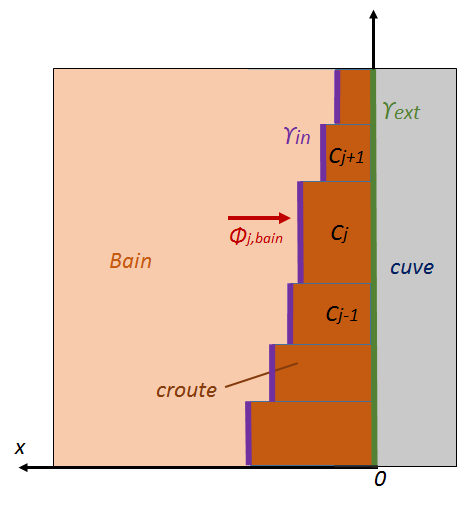
\includegraphics[width=0.4\textwidth]{Figures/crust_figure.png}
\caption{Schéma de la croûte couplée à au bain de corium liquide et de la cuve} \label{fig:crust_figure}
\end{figure}

Le domaine $\Omega_C$ est discrétisé en 1D selon la direction verticale (selon l'axe noté $z$) de la croûte. Le maillage est décrit par $N_{noeuds}$ noeuds. Les $N_{mailles}=N_{noeuds}-1$ mailles rectangulaires correspondantes sont notées $C_j$ pour $1 \leq j\leq N_{mailles}$. Pour chaque maille, la direction horizontale est donnée par l'axe $x$. On note [$x_j^{min}, x_j^{max}$] le domaine occupé par la maille $j$ suivant l'axe $x$ et $S_j$ la surface de la face verticale (i.e. suivant l'axe $z$). On fixera, comme indiqué sur la figure \ref{fig:crust_figure} $x_j^{min}=0,\forall j$. A chaque pas de temps, le bain de corium peut changer de configuration (e.g. stratification, baisse ou élévation du niveau du bain). Ainsi, à chaque pas de temps le domaine occupé par la croûte est remaillé à partir d'un pas d'espace de référence en respectant les contraintes suivantes :
\begin{itemize}
    \item une maille ne peut pas être en face de deux couches du bain, ainsi celle-ci ne recevra un flux thermique provenant uniquement d'une seul couche
    \item quelque soit l'épaisseur d'une couche du bain de corium, au moins une maille sera définie en face de cette couche
    \item  Il peut apparaître éventuellement au cours d'un calcul une autre partie de $\gamma_{in}$ située plus haut que le niveau supérieure du bain de corium liquide (e.g. lorsque le niveau du bain baisse, une partie de la croûte ne voit plus le corium liquide). Dans ce cas on considérera une condition adiabatique.
\end{itemize}
A chaque remaillage du domaine occupé par la croûte, une projection des masses et des températures est effectuée sur le nouveau maillage en assurant une conservation en masse et en énergie (voir section \ref{couplage}).\\

Les propriétés physiques liées à la croûte sont pour chaque maille $j$ : $T_j$ la température, $\rho_j$ la densité, $\lambda^s_j$ la conductivité thermique, $\heatCp[s]{j}$ la capacité thermique, $\Delta {\cal H}_j^{fus}$ l'enthalpie de fusion et $T_j^{fus}$ (resp. $\temperature[sol]{l(j)}$) la température de fusion de la croûte (resp. la température de solidification du corium liquide associé à la couche située en face de la maille $j$).

 Sur la frontière $\gamma_{in}$, une partie de la croûte est en contact avec le corium liquide, elle est alors soumise à un flux $\phi_{bain}$ provenant du bain de corium liquide. Sur la frontière $\gamma_{ext}$, une condition de température imposée ($T=T^{ext}$) ou de flux imposé ($\phi=\phi^{out}$) peut être définie.\\

Les quantités moyennes suivantes sont introduites pour $1 \leq j\leq N_{mailles}$ :
\begin{eqnarray}
m_{j}(t) &=& \rho_j  V_j(t) \\
\overline{T}_{j}(t) &=& \frac{1}{V_j(t)} \int_{C_j(t)} T_{j}(x,z,t)\,\mathrm{d}x\, \mathrm{d}z\\
\overline{h}_j(t) &=& \frac{1}{m_j(t)} \int_{C_j(t)} h_j(x,z,t)\,\mathrm{d}x\, \mathrm{d}z\\
\overline{\phi}_{j,in}(t) &=& \frac{1}{S_j}\int_{\gamma_{in}\cap S_j}\lambda_j^s \frac{\partial T_{j}}{\partial x}(x=x_j^{max},z,t)\, \mathrm{d}z  \label{eq:phi_j_in}\\
\overline{\phi}_{j,ext}(t) &=& \frac{1}{S_j}\int_{\gamma_{ext}\cap S_j}\lambda_j^s \frac{\partial T_{j}}{\partial x} (x=x_j^{min},z,t)\, \mathrm{d}z  \label{eq:phi_j_ext}
\end{eqnarray}
avec $T_{j}$ la température de la maille $j$, $h_j$ l'enthalpie spécifique et $V_j$ le volume de la maille $j$.\\

Le système (\ref{eq:mass})-(\ref{eq:enthalpie}) suivant donne l'évolution des masses et enthalpies spécifiques moyennes pour chaque maille $j$ :

\begin{eqnarray}
\frac{dm_{j}}{dt} &=& - \frac{dm_{j}^\text{fus/sol}}{dt} \label{eq:mass} \\ 
%m_{j} C_{p,C} \frac{d \overline{T}_{j}}{dt} &+& \frac{dm_{j}^\text{fus/sol}}{dt}C_{p,C} \left(T^{fus/sol} - \overline{T}_{j}\right) \\ &=& S_i\left(\overline{\phi}_{j,in} - \overline{\phi}_{j,ext}\right) + \dot{q}^m m_{j}
 \frac{d}{dt}(m_{j}\overline{h}_{j}) + \frac{dm_{j}^\text{fus/sol}}{dt} \overline{h}_{\gamma_{in},j} & = & S_i\left(\overline{\phi}_{j,in} - \overline{\phi}_{j,ext}\right) + \dot{q}^m m_{j} \label{eq:enthalpie}
\end{eqnarray}

où :

\begin{itemize}
 \item $\frac{dm_j^\text{fus/sol}}{dt}$ est le taux de masse ablatée dans le cas d'une fusion de la croûte ou le taux de masse solidifiée dans le cas d'une solidification du corium liquide. Ce taux de masse est positif dans le cas d'une fusion et négatif dans le cas d'une solidification;
 \item $\overline{h}_{\gamma_{in},j}$ représente l'enthalpie spécifique à l’interface $\gamma_{in}$ ;
 \item $\dot{q}^m m_j$ représente la contribution de la puissance résiduelle ($W$) associée à la puissance résiduelle massique $\dot{q}^m$ ($W/kg$);
\end{itemize}
Dans ce système, la conduction axiale (i.e. suivant l'axe $z$) a été négligée. Il est à noter qu'une option est disponible dans le code pour prendre en compte une approximation numérique de flux thermique axial (\cite{Peybernes2018}). 

Une maille $C_j$ peut être dans trois types "d'état" : soit elle est en fusion, soit en solidification, soit le volume de la maille $C_j$ reste constant. Dans ce dernier cas, on dira par la suite que la maille $C_j$ est en "pure conduction". Par la suite, en considérant que la température de la frontière interne de la croûte $\gamma_{in}$, que l'on note $T_{j,in}$, vérifie $\temperature[sol]{l(j)}\leq T_{j,in}\leq T_j^{fus}$, on supposera qu'une maille $C_j$ doit passer par un état de "pure conduction" pour passer d'un état de fusion à un état de solidification ou inversement.

En fonction des valeurs atteintes par $T_{j,in}$, les fermetures associées au système d'équations précédent prennent des formes différentes. Ci-dessous sont listés les différents cas de figure :\\

\begin{itemize}
\item {\it cas d'une pure conduction dans la croûte :}\\
Tant que $T_{j,in}<T_j^{fus}$, la fusion de la maille de croûte $C_j$ n'a pas commencé :
\begin{eqnarray*}
\frac{dm_j^\text{fus/sol}}{dt} &=& 0.0 \\
\overline{\phi}_{j,in} &=& \phi_{j,bain}
\end{eqnarray*}

\item {\it passage en fusion de la croûte :}\\
Si $T_{j,in}$ atteint la température $T_j^{fus}$ ($T_{j,in}\ge T_j^{fus}$), la fusion de la maille $C_j$ commence suivant l'équation de front de fusion suivante :
\begin{eqnarray*}
\Delta \mathcal{H}_j^{fus} \frac{dm_j^\text{fus/sol}}{dt} &=& S_j\left(\phi_{j,bain} - \overline{\phi}_{j,in}\right) \\
T_{j,in} &=& T_j^{fus}
\end{eqnarray*}

\item {\it passage en solidification du corium :}\\
Si $T_{j,in}$ atteint la température $\temperature[sol]{l(j)}$ ($T_{j,in}\le \temperature[sol]{l(j)}$), la solidification du corium commence suivant l'équation du front de solidification suivante :
\begin{eqnarray*}
\Delta \mathcal{H}_j^{fus} \frac{dm_j^\text{fus/sol}}{dt} &=& S_j\left(\phi_{j,bain} - \overline{\phi}_{j,in}\right) \\
T_j^{in} &=& \temperature[sol]{l(j)}
\end{eqnarray*}

\item {\it passage en conduction pure après un arrêt d'une fusion/solidification :}\\
Lorsque une maille $C_j$ est en fusion ou solidification, si $\frac{dm_i^\text{fus/sol}}{dt}$ s'annule, le front de fusion/solidification s'arrête. Et ainsi la maille $C_j$ devient en "conduction pure" :
\begin{eqnarray*}
\frac{dm_j^\text{fus/sol}}{dt} &=& 0.0 \\
\phi_j^{in} &=& \phi_{j,bain}
\end{eqnarray*}
\end{itemize}

En pratique, selon l'état de la maille $C_j$, il est nécessaire de compléter également l'équation d'énergie par des lois de de fermeture pour les quantités $\overline{\phi}_{j,in}$ and $\overline{\phi}_{j,ext}$. Pour ce faire, un modèle 0D basé sur l'hypothèse d'un profil quadratique suivant l'axe $x$ de la température permet de déduire ces $\overline{\phi}_{j,in}$ and $\overline{\phi}_{j,ext}$ \cite{LeTellier2016}.Lors de la résolution, selon l'état de la maille $C_j$, il est nécessaire de compléter également l'équation d'énergie par des lois de de fermeture pour les quantités $\overline{\phi}_{j,in}$ and $\overline{\phi}_{j,ext}$. Pour ce faire, un modèle 0D basé sur l'hypothèse d'un profil quadratique suivant l'axe $x$ de la température permet de déduire ces $\overline{\phi}_{j,in}$ and $\overline{\phi}_{j,ext}$ \cite{LeTellier2016}.\\

{\it Remarque :}
En pratique, à l'initialisation d'un calcul, un maillage de la croûte est défini à partir du nombre de mailles imposé par l'utilisateur et de la stratification du bain de corium. L'algorithme actuel ne prévoit pas d'avoir des mailles de croûte ne contenant aucun matériau. Ainsi, à l'initialisation d'un calcul ou lorsque une nouvelle maille de croûte apparaît en cours de calcul suite à une modification de la hauteur du bain, cette nouvelle maille de croûte est occupée par un "résidu" de matériau dont la composition est donnée par la couche du bain de corium en face de cette maille. Initialement, l'épaisseur de la maille $e_j^0$ est fixée par l'utilisateur. La masse $m_j^0$ est déduite à partir de cette épaisseur et de la densité du matériau. Concernant la température, on suppose qu'à l'initialisation de la maille de croûte, elle correspond à un état stationnaire avec ainsi un profil quadratique de la forme : 
$$T_j(x)=ax^2+bx+c.$$
A partir de l'équation de chaleur vérifiée en stationnaire et des deux conditions aux limites en $x=x_j^{min}=0$ et $x=e_j^0$, les coefficients $a$, $b$ et $c$ sont calculés. Par exemple pour une température fixée côté cuve en $x=0$ $(T_j^{ext})$ et une température de fusion fixée $T_j^{fus}$ en $x=e_j^0$ côté bain, ces coefficients obtenus prennent la forme :
\begin{eqnarray}
c &=& T^{ext}_j \\
b &=& \frac{T_j^{fus}-T^{ext}_j}{e_j^0}+\frac{\dot{q}^m m_j^0}{2\lambda_j^s S_j} \\
a &=& -\frac{\dot{q}^m m_j^0}{2\lambda_j^s e_j^0 S_j}
\end{eqnarray}

La température moyenne initiale de la maille $j$ est ainsi donnée par :
$$\overline{T}_{j}=\frac{a}{3} ({e_j^0})^2 + \frac{b}{2} e_j^0 + c$$

\subsection{Traitement de la composition de la croûte et fermetures thermodynamiques} \label{sect:thermochimie}

Dans cette première version du modèle de croûte, la gestion de la composition des mailles de croûtes et des fermetures ``thermodynamiques''\footnote{thermodynamique au sens de la description du système multicomposant par le biais de son énergie de Gibbs, à la manière de la méthode CALPHAD \cite{Lukas2007}} est volontairement simplifiée tout en préservant, autant que faire se peut, une description qualitativement correcte. Autrement dit, cette première version du modèle n'intègrent pas tous les résultats et développements associés à l'action (par ailleurs initiée dans le cadre de la fiche ``Modélisation en Accidents Graves'' du projet CORIU) d'utilisation consistante et exhaustive des données thermodynamiques d'une base CALPHAD dans les modèles de fond de cuve (voir \cite{LeTellier2016b,Tiwari2018,LeTellier2019}. Ces choix, ainsi que les perspectives d'amélioration dans une future version de ce modèle, sont discutés dans ce paragraphe.

Tout d'abord, la composition de la croûte (comme pour les différentes couches du bain ou des lits de débris) est décrite par le biais des fractions massiques des espèces. Seule une composition moyenne pour chaque maille $j$  (\textit{i.e.} $\left(\avMassFraction[i]{j}\right)_{i\in \speciesSet}$ où $\speciesSet$ est l'ensemble des espèces considérées) est suivie. La composition en éléments associée est notée $\left(\elementMassFraction[j]{}\right)_{i\in\elementSet}$.

Ensuite, du point de vue de l'enthalpie spécifique $\avMassEnthalpy{j}$, pour chaque maille $j$, elle est explicitement écrite en température et correspond formellement à la description suivante des enthalpies spécifiques du solide $\avMassEnthalpy[s]{j}$ et du liquide $\massEnthalpy[l]{j}$ associées à ce matériau :
\begin{eqnarray}
 \avMassEnthalpy{j} \left(\temperature{}\right) = \avMassEnthalpy[s]{j} \left(\temperature{}\right) &=& \massEnthalpy[o]{} - \heatCp[s]{j} \left(\temperature[fus]{j} - \temperature{}\right) \\
 \massEnthalpy[l]{j} \left(\temperature{}\right) &=& \heatCp[l]{j} \left(\temperature{} - \temperature[fus]{}\right) + \dEnthalpy[fus]{j} + \massEnthalpy[o]{}
\end{eqnarray}
où $\massEnthalpy[o]{}$ est une enthalpie de référence et les capacités calorifiques $\heatCp[s]{j}$, $\heatCp[l]{j}$ et la chaleur latente de fusion $\dEnthalpy[fus]{j}$ sont évaluées, comme pour les phases du bain de corium ou les débris, par le biais de l'interface disponible dans PROCOR aux lois de propriétés physiques par espèces et des lois de mélanges implantées TOLBIAC-ICB.

Pour ce qui est des températures de solidification $\temperature[sol]{l(j)}$ et de fusion $\temperature[fus]{j}$ associées aux possibles changement de condition à l'interface entre la maille $j$ et la couche du bain correspondante $l(j)$ (voir \Sect{thermique}), on considère que :
\begin{itemize}
 \item la fusion de la maille $j$ a lieu à $\temperature[fus]{j}=\Mc{T}_{liq}\left(\elementMassFraction[j]{}\right)_{i\in\elementSet}$, la température de liquidus associée à la composition élementaire de la maille de croûte $j$ ;
 \item la solidification de la couche $l(j)$ a lieu à $\temperature[sol]{l(j)}=\Mc{T}_{liq}\left(\elementMassFraction[l(j)]{}\right)_{i\in\elementSet}$, la température de liquidus associée à la composition élementaire de la couche du bain $l(j)$.
\end{itemize}
Lorsque la solidification a lieu, la composition du solide formé est prise égale à celle de la couche liquide. 

Ce traitement simplifié des fermetures thermodynamiques relatives à l'interface bain/croûte diffère de celles obtenues sous l'hypothèse d'équilibre local dans le modèle consistant avec une base CALPHAD décrit dans \cite{Tiwari2018}. Comme évoqué plus haut, cette simplification est volontaire à ce stade du développement et du test de ce modèle de croûte. Ainsi, le ``branchement'' dans ce modèle de l'équation d'état dédiée au corium en cuve construite dans le cadre de la fiche ``Modélisation en Accidents Graves'' se fera dans un second temps. Pour autant, par un choix adéquat des températures de liquidus, ce traitement simplifié permet de conserver qualitativement (et très probablement quantitativement, au premier ordre) le comportement attendu du couplage entre ce modèle de croûte et le modèle de bain stratifié.

Pour discuter le choix de ces fermetures associées aux températures de liquidus, quelques calculs d'équilibre thermodynamique réalisés pour différents mélanges entre du corium sous-oxydé (système U-O-Zr) et de l'acier (ici réduit à Fe) sont présentés au \Tab{liquidus} ; les mélanges retenus sont typiques des compositions rencontrées pour les réacteurs à eau pressurisée. Les calculs ont été réalisés avec Open-Calphad pour le système quaternaire U-O-Zr-Fe tel que décrit dans la base NUCLEA'09. En plus de la température de liquidus relative à l'inventaire complet (noté ``global'' au \Tab{liquidus}), les températures de liquidus des deux phases liquides (une ``oxyde'' et une ``métal'') prédites par un calcul d'équilibre à 2900K (température à laquelle toutes ces compositions sont dans la lacune de miscibilité liquide du système U-O-Zr-Fe) ont été évalués. De manière cohérente, pour chaque composition, les températures de liquidus pour les inventaires ``global'', ``oxyde'' et ``métal'' sont quasiment identiques et toujours associées à l'apparition de la phase solide cubique face centrée (U,Zr)O$_{2-x}$ (notée \T{C1\_FCC}). On remarquera aussi que, dans la phase liquide métallique, le quantité d'O ``disponible'' pour former ce solide réfractaire est très faible, de l'ordre de quelques kilos par tonne de liquide. Si l'on considère la solidification sous l'hypothèse d'un équilibre local à l'interface de cette phase métallique, on observerait donc la formation très limitée et négligeable d'un solide réfractaire. Une fois l'oxygène ``épuisé'', comme le calcul de température de liquidus pour l'inventaire ``métal sans O'' l'illustre, la solidification ne peut intervenir qu'à une température beaucoup plus basse (associée à la formation d'une phase de Laves (composés intermétalliques, notée (notée \T{LAVES})).

Ainsi, de manière cohérente, pour une fermeture simplifiée de notre système d'équations, on pourra retenir, sous l'hypothèse d'une solidification à la composition de liquide, la simplification suivante pour $\Mc{T}_{liq}\left(\elementMassFraction[j]{}\right)_{i\in\elementSet}$ :
\begin{equation}
 \Mc{T}_{liq}\left(\elementMassFraction[j]{}\right)_{i\in\elementSet} = 
 \left\{\begin{array}{rcl} \temperature[oxy]{liq} & & \text{pour une phase ``oxyde''} \\
                           \temperature[steel]{liq} & & \text{pour l'acier} \\
                           \temperature[met]{liq} & & \text{pour une phase métallique enrichie en U, Zr} 
 \end{array}\right.
\end{equation}
où $\temperature[oxy]{liq}$ de l'ordre de 2800-3000K, $\temperature[steel]{liq}$ de l'ordre de 1700-1800K et $\temperature[met]{liq}$ de l'ordre de 1500-1600K.

\begin{remark}
  Dans un contexte d'évaluation de la rétention du corium en cuve où l'on cherche en premier lieu à évaluer le risque de percement en transitoire par ``focusing effect'', la solidification à l'interface d'une phase métallique n'aura pas lieu et l'on est pas sensible à la valeur exacte de la température $\temperature[met]{liq}$. Cette fermeture redevient significative si l'on considère des temps plus longs (auxquels le bain de corium a suffisamment refroidi) pour l’évaluation de la rétention à long terme du corium dans la cuve. Pour cette application, la modélisation présentée est incomplète et devra être complétée en premier lieu par l'interfaçage de ce modèle avec l'équation d'état dédiée au corium en cuve construite dans le cadre de la fiche ``Modélisation en Accidents Graves''. Par ailleurs, du point de vue des fermetures discutées dans ce paragraphe, le choix d'une représentation uniforme de la composition de la croûte dans chacune des mailles sera sûrement invalidée et, tenir compte, \textit{a minima} au travers d'une représentation radiale à deux zones dans chaque maille axiale, du changement de phase solide formée (\T{C1\_FCC}, \T{LAVES}) semble nécessaire.
\end{remark}

\begin{table}[H]
\caption{Températures de liquidus et compositions associées à des calculs d'équilibre thermodynamique dans la lacune de miscibilité à 2900K}\label{tab:liquidus}
 \begin{tabularx}{\textwidth}{|c|c|C|C|C|C|} \cline{3-6}
 \multicolumn{2}{c|}{} & \multicolumn{2}{c|}{$R_{U/Zr}=1.2$ et $C_{Zr}=0.3$} & \multicolumn{2}{c|}{$R_{U/Zr}=1.2$ et $C_{Zr}=0.3$} \n \hline
 \multicolumn{2}{|c|}{$x_{steel}$} & $0.2^\dagger$ & $0.5^\ddagger$ & $0.05^\dagger$ & $0.2^\ddagger$ \n \hline
 \multirow{4}{*}{\rotatebox{90}{$\Mc{T}_{liq}$ (K)}} & global & 2831 & 2843 & 2841 & 2853 \n
  & oxyde  & 2830 & 2843 & 2841 & 2853 \n
  & métal  & 2829 & 2842 & 2840 & 2852 \n
  & métal sans O & 1620 & 1479 & 1581 & 1547 \n \hline
 \multirow{4}{*}{\rotatebox{90}{métal}} & $\elementMassFraction[U]{}$ & 0.416 & 0.278 & 0.389 & 0.252 \n  
 & $\elementMassFraction[Zr]{}$ & 0.115 & 0.070 & 0.101 & 0.057 \n  
 & $\elementMassFraction[O]{}$ & 0.003 & 0.003 & 0.003 & 0.002 \n  
 & $\elementMassFraction[Fe]{}$ & 0.466 & 0.649 & 0.507 & 0.689 \n  \hline
 \end{tabularx}
 \begin{legend}
  $R_{U/Zr}$ & rapport molaire U/Zr \n
  $C_{Zr}$ & degré d'oxydation molaire du Zr \n
  $x_{steel}$ & rapport massique entre acier et coriul sous-oxydé \n
  $^\dagger$ & en-dessous du seuil d'inversion de stratification \n
  $^\ddagger$ & au-dessus du seuil d'inversion de stratification
 \end{legend}
\end{table}

\subsection{Couplage avec le bain de corium}\label{couplage}
Dans le modèle transitoire de stratification de bain de corium en fond de cuve de PROCOR, jusqu'à quatre couches sont considérées comme montré dans la figure \ref{fig:bain_corium_croute}. 
\begin{figure}
\centering
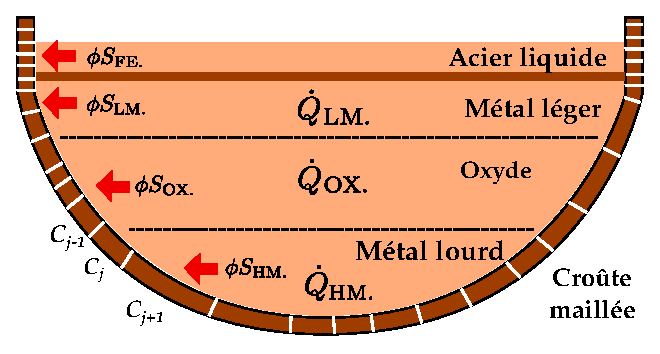
\includegraphics[width=0.7\textwidth, keepaspectratio=true]{Figures/bain_corium_croute.eps}
\caption{Bain de corium et sa croûte en fond de cuve.}
\label{fig:bain_corium_croute}
\end{figure}
De bas en haut peuvent exister une couche de métaux lourds (HM.), une couche d'oxydes (OX.) et une couche de métaux légers (LM.). Dans le modèle de stratification utilisé, la couche de métaux légers apparaît suite aux métaux remontant au travers de la couche d'oxydes lorsque le système à l'équilibre correspond à une couche de métaux légers au dessus d'une couche d'oxydes. Suivant des hypothèses de phénomènes de ségrégation de phase, ces trois couches sont entourées d'une croûte réfractaire. Une couche d'acier liquide hors équilibre (FE.), correspondant à la couche de \textit{focusing effect}, peut se trouver au dessus de ces trois couches. Seule la croûte en contact avec la cuve est modélisée dans cette note; la croûte en dessous de la couche d'acier liquide hors équilibre n'est pas modélisée par le modèle présenté et est seulement considérée en termes de fermeture pour la température entre le bain sous la croûte et cette couche. 

Les puissances résiduelles $\dot{\mathcal{Q}}$ (W) des couches métal lourd, oxyde et métal léger sont transmises, entre autres, latéralement aux mailles de la croûte sous forme de flux de chaleur $\phi S$ (W) par couche.

À l'interface entre une maille de croûte et la couche du bain correspondante, la température dépend de l'état thermique de la croûte. Si la croûte est en conduction, la température d'interface est donnée par l'égalité des flux de chaleur de part et d'autre de l'interface. Si la croûte est en fusion (resp. solidification), la température d'interface est donnée par la température de \textit{liquidus} (resp. \textit{solidus}). La température de \textit{solidus} de la croûte est donnée par la température de \textit{liquidus} de la couche de bain correspondante. Dans le modèle actuel de bain, les températures de \textit{liquidus} des trois couches de bain sous la croûte sont identiques et sont données par la température de \textit{liquidus} du bain homogène. Pour élargir le champ des possibilités, on fixera dans la note une température de \textit{liquidus} différente pour chaque couche. Pour plus de détails, voir la description du modèle de thermochimie dans la section précédente. 

Le couplage entre le modèle de bain de corium et le modèle de croûte se définit en termes d'échanges de données. De manière générale, que la croûte soit en conduction, en fusion ou en solidification, le modèle de bain de corium et le modèle de croûte échangent un flux de chaleur, une température d'interface et un débit de masse. Le couplage peut être défini sous la forme d'un graphe (voir le graphe de la figure \ref{fig:graphe_couplage_corium_croute}). 
\begin{figure}
\centering
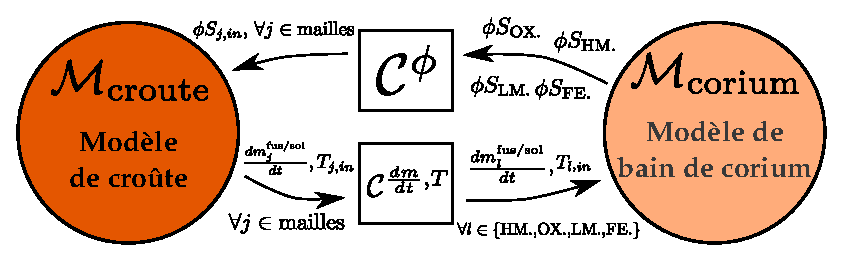
\includegraphics[width=0.7\textwidth, keepaspectratio=true]{Figures/graphe_couplage_corium_croute.eps}
\caption{Graphe du couplage entre le modèle de bain de corium et le modèle de croûte.}
\label{fig:graphe_couplage_corium_croute}
\end{figure}
Les modèles sont représentés par les n\oe{}uds du graphe et les échanges de données par des arcs entre les n\oe{}uds. Chaque arc contient un communicateur $\mathcal{C}$ permettant de faire communiquer \emph{correctement} des modèles qui, a priori, peuvent avoir des sorties et des entrées qui doivent être adaptées. Par exemple, le communicateur $\mathcal{C}^{\phi}$ permet de \emph{projeter} les puissances $\phi S$ par couche du bain en puissance $\phi S_j$ sur les multiples mailles $C_j$ de la croûte. De même, le communicateur $\mathcal{C}^{\frac{dm}{dt}, T}$ projette les débits de masse $\dot{m}_j$ et les températures d'interface $T_j$ par maille de croûte sur les couches du bain. 

La représentation par graphe et modèles et communicateurs est celle adoptée dans la plate-forme PROCOR pour le couplage. On ne donnera pas plus de détails sur l'aspect logiciel du couplage dans PROCOR. Plus de détails sur l'architecture et les algorithmes de couplage dans PROCOR peuvent être trouvés dans \cite{Viot2018}. En revanche, l'aspect numérique des communications est détaillé ci-après, en particulier les opérateurs mathématiques de projection et de réduction utilisés dans les communicateurs.

La projection d'un flux $phi$ d'une couche du bain 

\section{Résultats numériques}
Le bain initial correspond à un bain oxyde avec une masse initiale de 10 T, une température initiale de 2900 K et une composition de 0.77 UO$_2$ - 0.12 Zr - 0.11 ZrO$_2$ (ratio molaire $R_{U/Zr}$ = 1.3 et degré d'oxydation du zirconium $C_{Zr}$ = 30 \%). La puissance résiduelle constante $\dot{\mathcal{Q}} = 200$ MW est portée par l'espèce uranium U. Une condition adiabatique est imposée sur la couche d'acier liquide hors équilibre du bain (FE.), sinon, pour le bain sous la croûte, la température d'interface pour la couche supérieure est la température de fusion de la croûte. Les propriétés physiques des couches du bain sont calculés en fonction de la composition et de la température de la couche par un code externe. Enfin, les caractéristiques utiles des différentes couches du bain sont détaillées dans le tableau~\ref{tab:caracteristiques_couches_bain}, en particulier les températures de \textit{liquidus} $T^{fus}$ ainsi que les corrélations de flux de chaleur utilisées pour le calcul des puissances latérales $\phi S$ (voir~\cite{Bonnet1999} ou~\cite{Tourniaire2009a} pour plus de détails sur les corrélations).
\begin{table}
	\centering
	\begin{tabular}{ccc} 
	\hline
	Couche & $T^{fus}$ (K) & Corrélation latérale\\
	\hline
	Acier liquide (FE.) & 1600 & ChurchillAndChu\\
	Métal léger (LM.) & 1600 & ChurchillAndChu\\
	Oxyde (OX.) & 3000 & BaliDownWard\\
	Métal lourd (HM.) & 1600 & BaliDownWard\\
	\hline
	\end{tabular}	
	\caption{Configuration initiale du bain de corium pour le test.} 
	\label{tab:caracteristiques_couches_bain}
\end{table}
Un profil de flux plat est utilisé pour la projection des flux des différentes couches du bain sur les mailles de le croûte (voir section~\ref{couplage}).

Enfin, la croûte est divisée, tout au long du calcul, en 20 mailles. La puissance résiduelle constante $\dot{\mathcal{Q}} = 200$ MW dans la croûte est portée par l'espèce uranium U. Le résidu d'apparition de la croûte est de 5 mm. Une température constante et uniforme de 1800 K est imposée sur les parois extérieures de la croûte (seul le couplage entre le modèle de bain de corium et le modèle de croûte sont testés ici).

Différentes coulées d'acier liquide à différents instants du calcul permettent de reproduire des stratifications du bain d'intérêt pour les calculs accidents graves. En particulier, ces coulées ont été calculées en fonction du seuil d'inversion de stratification du bain (correspondant à quantité d'acier dans la bain permettant le passage d'un état d'équilibre thermochimique composé d'une couche de métaux lourds en dessous d'une couche d'oxydes vers un équilibre composé d'une couche d'oxydes en dessous d'une couche de métaux légers). Les caractéristiques de ces coulées (temps de début et de fin, masse, température et composition) sont détaillés dans le tableau~\ref{tab:coulees_acier}. 
\begin{table}
	\centering
	\begin{tabular}{ccccc} 
	\hline
	$t_{\text{début}}$ (s) &  $t_{\text{arrêt}}$ (s) & Débit (kg/s) & T (K) & Composition\\
	\hline
	15 000 & 15 200 & 5 & 1605 & 0.687 Fe - 0.208 Cr - 0.106 Ni\\
	30 000 & 30 200 & 8 & 1605 & 0.687 Fe - 0.208 Cr - 0.106 Ni\\
	\hline
	\end{tabular}	
	\caption{Les différentes coulées d'acier liquide imposées pour le test.} 
	\label{tab:coulees_acier}
\end{table}
Un temps suffisament long entre chacune de ces coulées est imposé pour permettre au bain d'atteindre un état quasi-stationnaire de thermique et de thermochimie. Les différentes configurations quasi-stationnaires du bain obtenues (OX. puis HM./OX. puis OX./LM.) sont décrites dans la figure~\ref{fig:stratification_bains}.
\begin{figure}
\centering
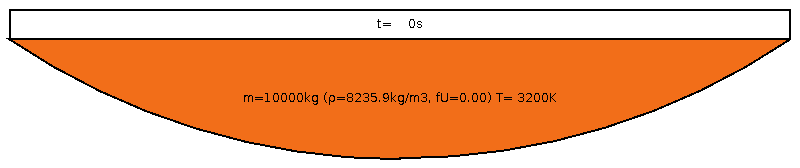
\includegraphics[width=0.8\textwidth, keepaspectratio=true]{Figures/coriumPool_t=00000.png}\\
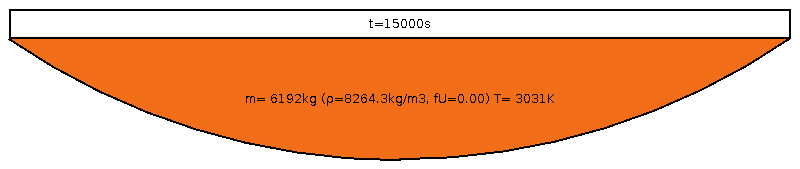
\includegraphics[width=0.8\textwidth, keepaspectratio=true]{Figures/coriumPool_t=15000.png}\\
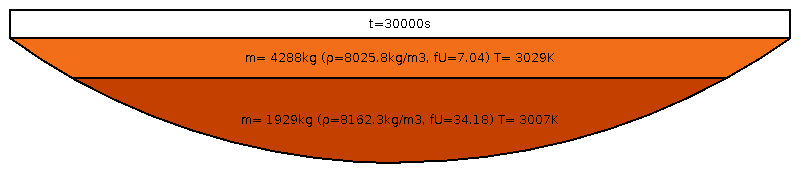
\includegraphics[width=0.8\textwidth, keepaspectratio=true]{Figures/coriumPool_t=30000.png}\\
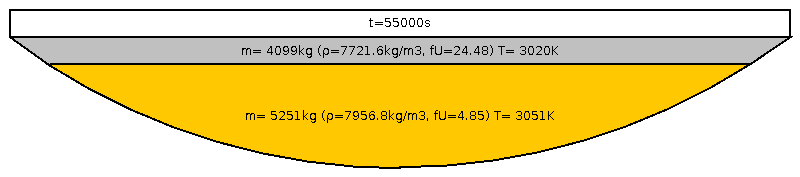
\includegraphics[width=0.8\textwidth, keepaspectratio=true]{Figures/coriumPool_t=55000.png}
\caption{La configuration initiale et les différentes stratifications quasi-stationnaires du bain de corium en fond de cuve atteintes lors du test : \textcolor{orange!75!black}{\textbf{OX.}} à t=15 000 s puis \textcolor{red!50!black}{\textbf{HM.}}/\textcolor{orange!75!black}{\textbf{OX.}} à t=30 000 s puis \textcolor{orange!75!black}{\textbf{OX.}}/\textcolor{orange!50!white}{\textbf{LM.}} à t=55 000 s.}
\label{fig:stratification_bains}
\end{figure}
On notera que, comme le montre la figure, le volume de la croûte est bien pris en compte pour le calcul du volume qu'occupe le bain de corium en fond de cuve de sorte que, hormis lors des coulées d'acier, le mouvement du bain reste relativement faible (et principalement dû aux propriétés physiques dépendantes de la température).

Par la suite, les premiers macro pas de temps du calcul ne seront pas considérés. Bien que l'initialisation thermique de la croûte expliquée dans la section~\ref{sect:thermique} permette d'obtenir un flux externe de croûte initialement, la configuration du couplage thermique entre le bain de corium et la croûte amène le modèle de conduction 0D utilisé à sur-évaluer ce flux externe sur les pas de temps suivants. Néanmoins, au bout de quelques pas de temps après épaississement de la croûte, le modèle de conduction évalue correctement les différents flux de chaleur de la croûte. On notera que ces problèmes causés par le modèle de conduction utilisé dans PROCOR ont déjà été identifiés dans une étude sur la prise en compte de la conduction axiale dans ce modèle dans~\cite{Peybernes2018}.

Durant les différentes étapes du transitoire, de la masse est échangée entre le bain de corium et sa croûte par solidification du bain ou fusion de la croûte. À chaque macro pas de temps du calcul et en fin de calcul, \emph{on vérifie bien la conservation de la masse globale du système}.

De la même manière, de l'énergie est échangée entre le bain de corium et la croûte et \emph{on vérifie la conservation globale de l'énergie du système}. La figure~\ref{fig:thermal_balance} donne les différentes puissances d'intérêt du bain de corium et de la croûte au cours du transitoire.
\begin{figure}
\centering
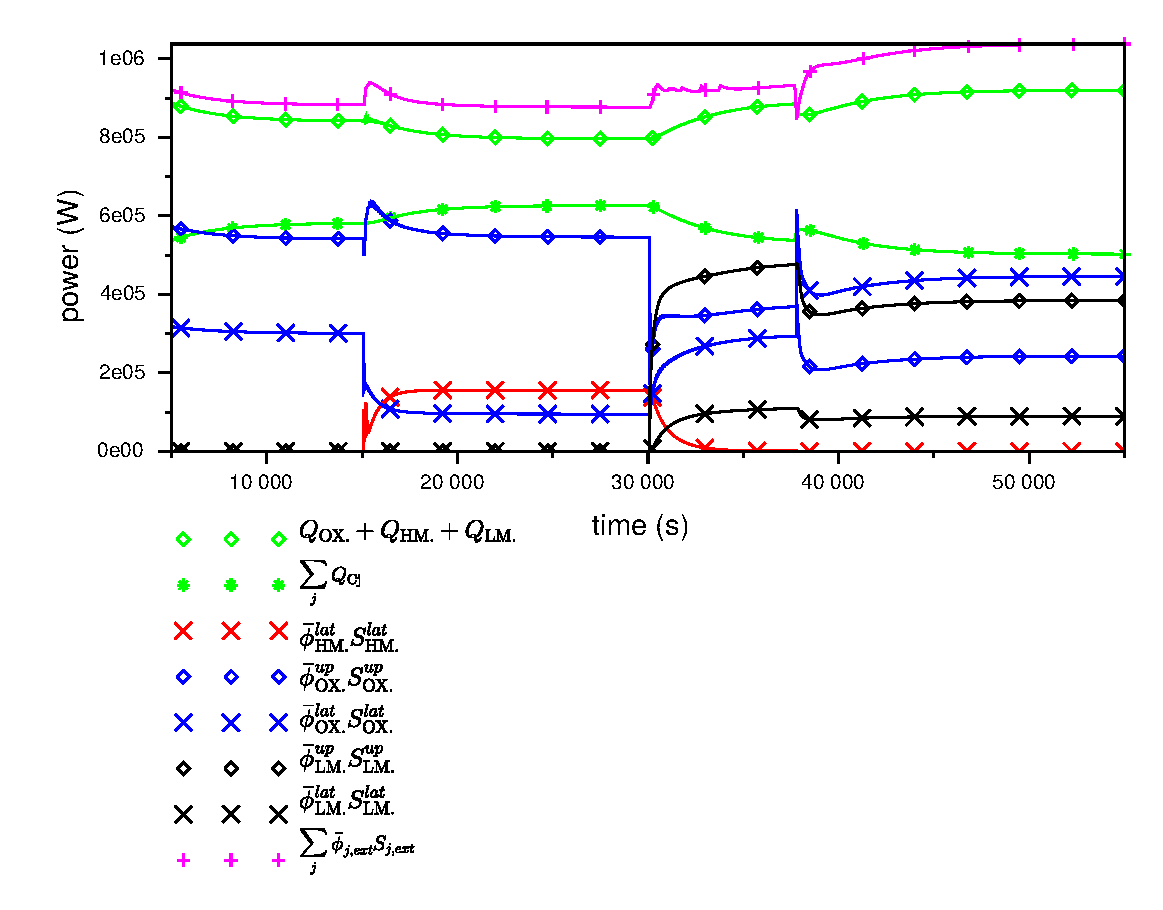
\includegraphics[width=0.85\textwidth, keepaspectratio=true]{Figures/thermal_balance.eps}\\
\caption{Puissances d'intérêt du système bain de corium et croûte.}
\label{fig:thermal_balance}
\end{figure}
En particulier, les puissances évacuées par les surfaces latérales des différentes couches du bain 
\begin{equation*}
\bar{\phi}^{lat}_\textrm{HM.}S^{lat}_\textrm{HM.},\,\bar{\phi}^{lat}_\textrm{OX.}S^{lat}_\textrm{OX.},\,\bar{\phi}^{lat}_\textrm{LM.}S^{lat}_\textrm{LM.}
\end{equation*}
et par sa surface supérieure 
\begin{equation*}
\bar{\phi}^{up}_\textrm{OX.}S^{up}_\textrm{OX.}\quad\text{puis}\quad\bar{\phi}^{up}_\textrm{LM.}S^{up}_\textrm{LM.}\quad\text{pour t $>$ 30 000 s},
\end{equation*}
la somme des puissances résiduelles des couches du bain $Q_\textrm{OX.}+Q_\textrm{HM.}+Q_\textrm{LM.}$ ainsi que la somme des puissances résiduelles $Q_{C_j}$ des mailles $C_j$ de la croûte, et enfin la somme des puissances $\bar{\phi}_{j,ext}S_{j,ext}$ évacuées par la surface extérieure $\gamma_{ext}$ des mailles $C_j$ de la croûte. La conservation de l'énergie peut être vérifiée graphiquement dans la figure~\ref{fig:thermal_balance} aux trois états quasi-stationnaires atteints. Par exemple, pour t=15 000 s, on a :
\begin{equation}
\bar{\phi}^{up}_\textrm{OX.}S^{up}_\textrm{OX.} + \bar{\phi}_{j,ext}S_{j,ext} = Q_\textrm{OX.} + \sum_j Q_{C_j}.
\end{equation}

Durant le transitoire, les mailles de la croûte passent dans les différents états décrits dans la section~\ref{sect:thermique} (solidification, conduction et fusion). En particulier, pour la première partie du transitoire pour t $\leq$ 15 000 s, la croûte se solidifie jusqu'à atteindre un état quasi-stationnaire de solidification (voir figure~\ref{fig:croutes_1}).  
\begin{figure}
\centering
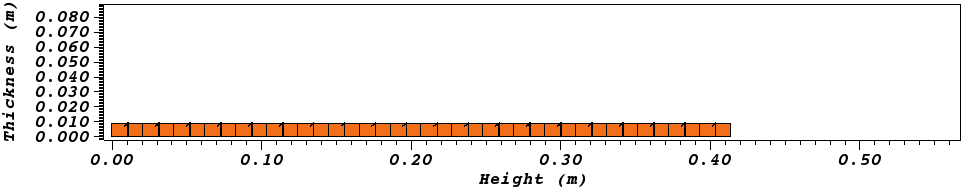
\includegraphics[width=\textwidth, keepaspectratio=true]{Figures/croute_100.png}\\
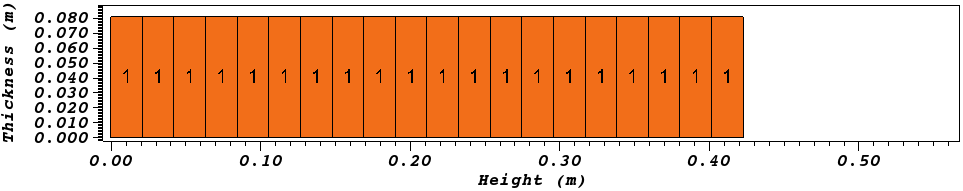
\includegraphics[width=\textwidth, keepaspectratio=true]{Figures/croute_15000.png}
\caption{Croûte à t = 100 s (en haut) et à t = 15 000 s (en bas). \textit{L'indice dans la maille $C_j$ donne la couche de bain en face de celle-ci : 0 $\Leftrightarrow$ HM., 1 $\Leftrightarrow$ OX., 0 $\Leftrightarrow$ LM., 3 $\Leftrightarrow$ FE., -1 $\Leftrightarrow$ pas de contact avec le bain}.}
\label{fig:croutes_1}
\end{figure}

Lors de la seconde partie du transitoire, la couche de métal lourd apparaît suite à une coulée d'acier liquide (voir tableau~\ref{tab:coulees_acier}). La figure~\ref{fig:croutes_2} donne les différents états de la croûte durant ce transitoire.
\begin{figure}
\centering
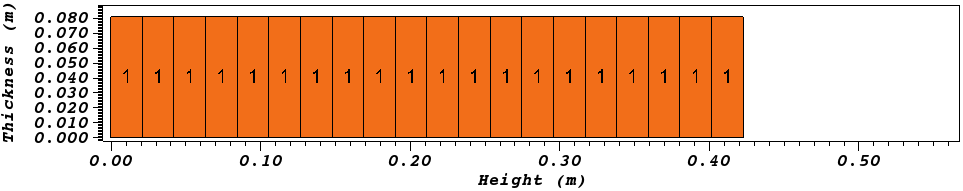
\includegraphics[width=\textwidth, keepaspectratio=true]{Figures/croute_15000.png}\\
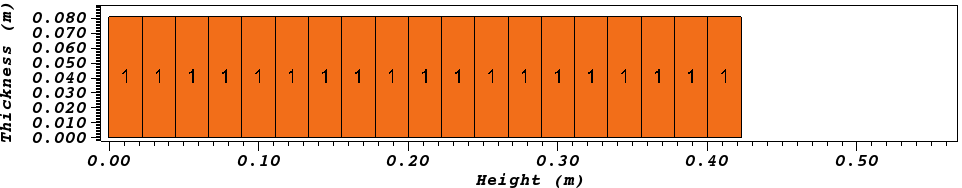
\includegraphics[width=\textwidth, keepaspectratio=true]{Figures/croute_15100.png}\\
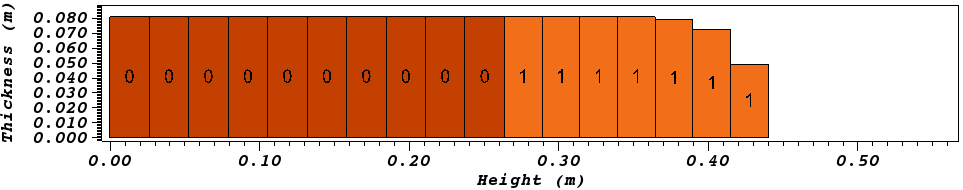
\includegraphics[width=\textwidth, keepaspectratio=true]{Figures/croute_16000.png}\\
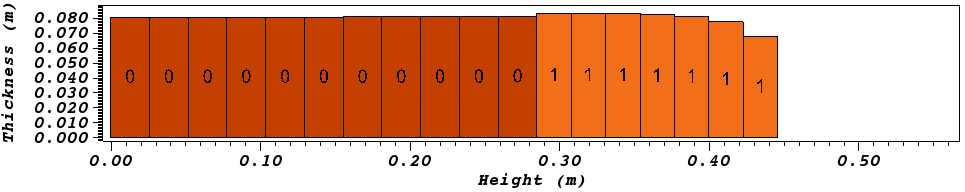
\includegraphics[width=\textwidth, keepaspectratio=true]{Figures/croute_18000.png}\\
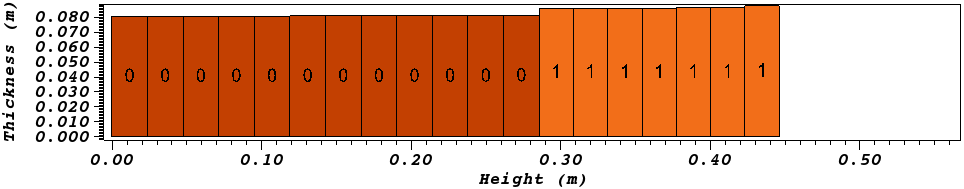
\includegraphics[width=\textwidth, keepaspectratio=true]{Figures/croute_30000.png}\\
\caption{De haut en bas, croûte à t = 15 000 s, t=15 100 s, t=16 000 s, t=18 000 s, t=30 000 s (état quasi-stationnaire du bain HM./OX.). \textit{L'indice dans la maille $C_j$ donne la couche de bain en face de celle-ci : 0 $\Leftrightarrow$ HM., 1 $\Leftrightarrow$ OX., 0 $\Leftrightarrow$ LM., 3 $\Leftrightarrow$ FE., -1 $\Leftrightarrow$ pas de contact avec le bain}.}
\label{fig:croutes_2}
\end{figure}
Entre t=15 000 s et t=15 100 s, une maille de croûte apparaît en face d'une couche d'acier liquide (à une hauteur h $>$ 0.42 m) provenant de la coulée et le maillage de la croûte oxyde passe de 20 mailles (à t=15 000s) à 19 mailles (à t=15 100s). Cette maille de croûte acier apparaît avec une épaisseur initiale de 5 mm mais fond presque instantanément et disparaît. Ensuite, la couche de métal lourd s'épaissit et le volume du bain augmente du fait des propriétés physiques différentes des couches HM. et OX.. Par conséquent, une croûte oxyde apparaît au fur et à mesure (voir les figures à t=16 000 s et t=18 000 s). À t=30 000 s, la thermochimie et la thermique du bain se sont stabilisées et la croûte n'évolue plus : on retrouve bien les profils plats de flux projetés sur les mailles de la croûte.

Enfin, la figure~\ref{fig:croutes_3} donne l'évolution de la croûte pour la dernière partie du transitoire entre t=30 000 s et t=55 000 s.
\begin{figure}
\centering
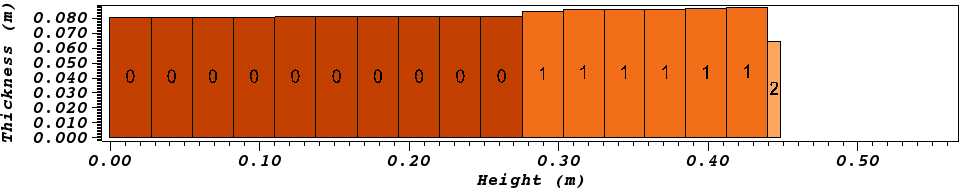
\includegraphics[width=\textwidth, keepaspectratio=true]{Figures/croute_30200.png}\\
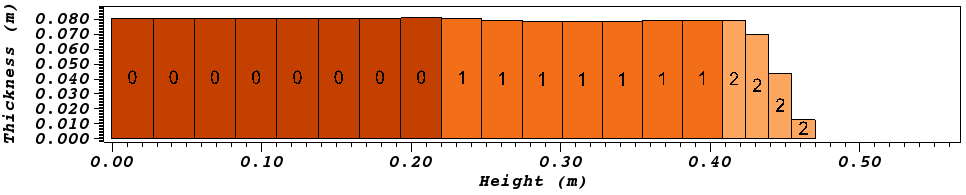
\includegraphics[width=\textwidth, keepaspectratio=true]{Figures/croute_31000.png}\\
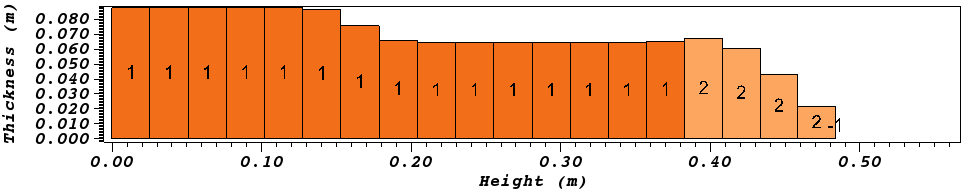
\includegraphics[width=\textwidth, keepaspectratio=true]{Figures/croute_38000.png}\\
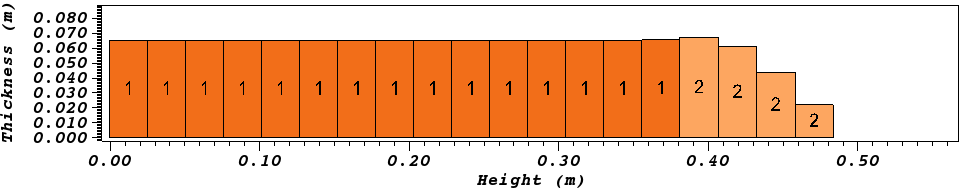
\includegraphics[width=\textwidth, keepaspectratio=true]{Figures/croute_55000.png}
\caption{De haut en bas, croûte à t = 30 200 s, t=31 000 s, t=38 000 s, t=55 000 s (état quasi-stationnaire du bain OX./LM.). \textit{L'indice dans la maille $C_j$ donne la couche de bain en face de celle-ci : 0 $\Leftrightarrow$ HM., 1 $\Leftrightarrow$ OX., 0 $\Leftrightarrow$ LM., 3 $\Leftrightarrow$ FE., -1 $\Leftrightarrow$ pas de contact avec le bain}.}
\label{fig:croutes_3}
\end{figure}
On peut voir l'apparition d'une première maille de croûte en face de la couche métal léger LM. du bain (indice 2 dans la figure). Le volume du bain augmente suite aux coulées d'acier et plusieurs mailles de croûte en face de la couche LM. apparaissent. À t=38 000 s, suite à l'inversion de stratification du bain, la couche de métal lourd HM. disparaît au profit d'une couche oxyde OX.. Par conséquent, les mailles de croûte plus froide précédemment en face de celle-ci passent de l'état conduction à l'état solidification ($\temperature[sol]{HM.} < \temperature[sol]{OX.}$). À t=38 000 s, les premières mailles de croûte sont suffisamment chauffées et repassent en fusion jusqu'à atteindre un état stationnaire à t=55 000 s avec un profil de flux plat du bain.



\section{Conclusion}
Dans le cadre de l'amélioration de la modélisation du comportement du corium en fond de cuve, ce rapport propose un modèle permettant la prise en compte explicite d'une croûte située à l'interface d'un bain de corium avec la cuve. Pour ce faire, un maillage 1D de la croûte est introduit pour la résolution des équations d'évolution en masse et énergie. Le déplacement du front de fusion/solidification est traité par un modèle de Stefan. En fonction de la température à l'interface entre le bain et la croûte, l'algorithme développé permet à chaque maille de croûte d'être soit en fusion, soit en solidification, soit dans un état dans lequel seule la conduction est considérée lorsque la température d'interface se situe entre une température de solidification et de fusion. La température de fusion est donnée par la température de liquidus associée à la composition de la croûte, tandis que la température de solidification est donnée par la température de liquidus associée à la composition de la couche du bain qui est en contact. 

En fonction du changement de configuration du bain (stratification, hauteur), un remaillage est réalisé afin de permettre un couplage pertinent entre la croûte et le bain assurant un transfert thermique rigoureux entre les mailles de croûte et les couches du bain. Les masses et les énergies associées au nouveau maillage sont assurées par une projection conservative de ces quantités. Le couplage en temps est assuré par la plateforme PROCOR à l'aide d'une représentation par graphe des modèles et communications de données (flux thermiques, températures, débits de masse).\\

Une application numérique, de l'ordre du test de vérification du modèle, est présentée dans ce document pour illustrer le couplage entre le modèle de croûte et celui du bain de corium. Les résultats obtenus permettent de vérifier le bon comportement du modèle dans le cas de la solidification à l'interface d'un bain homogène oxyde. Lors de l'apparition  subséquente d'une phase métallique en contact avec la croûte oxyde (associée au transitoire de stratification), de par le choix d'une modélisation distinguant des températures de solidification et de fusion différentes à l'interface, le cas test présenté a mis en lumière des oscillations non-physiques associées au schéma de couplage explicite et, eventuellement, aux fermetures du bilan thermique de la croûte (approximation des flux conductifs). Cette pathologie requiert une analyse plus détaillée afin de pouvoir fournir une première version satisfaisante du modèle couplé avec un bain stratifié. Elle sera réalisée par le biais d'un cas test proposé dans cette note. \\

La suite directe du travail rapporté ici est le test de ce modèle sur des applications réacteurs et la comparaison avec les résultats obtenus avec le modèle de bain initial de PROCOR avec une croûte ``fictive''. Ce travail sera réalisé en 2019 dans le cadre du projet IVMR avec une reprise des benchmarks étudiés dans le WP2.2 et une nouvelle série de calculs réacteurs dans le WP2.5.

En perspectives du travail de modélisation, une évolution du modèle proposé dans ce rapport est le traitement de la conduction dans la croûte en 2D (et non plus seulement radiale). Ce développement se justifie lorsque l'épaisseur de croûte devient suffisamment épaisse pour que la conduction dans la direction axiale puisse avoir un effet. Ce cas de figure peut arriver aux temps longs, lorsque le bain de corium se refroidit significativement et que la masse de solide devient importante, mais également aux temps courts où la croûte est plus épaisse dans la partie inférieure du fond de cuve. Le travail d'analyse des expériences de thermohydraulique des bains (e.g. LIVE) qui sera initié en 2019 dans le cadre de la fiche ``Modélisation des accidenst graves'' du projet CORIU permettra de fournir des éléments de validation de ce modèle de croûte et, le cas échéant, de préciser les conditions dans lesquelles la conduction 2D devient importanet à prendre en compte.

Par ailleurs, une étude complémentaire sera menée afin d'évaluer l'approximation dans les codes 0D consistant à prendre une température moyenne à l'interface de la couche mince métallique située en surface (température moyenne typiquement prise à la température de fusion de la cuve). En effet, lorsque la configuration du bain évolue, une portion de croûte issue de la solidification de la couche oxyde peut se retrouver sur une partie de l'interface de la couche métallique. Le bain de corium peut ainsi être à la fois en contact avec la croûte sur une partie de l'interface et avec la cuve sur une autre portion. Des études avec un code de CFD seront réalisées pour estimer l'effet de cette variation de température à l'interface.


\bibliographystyle{elsarticle-num}
\bibliography{lma-jabref}
\end{document}
